\documentclass[a4paper,12pt]{thesis} % 修論・卒論など (ページが右端にでる)   

\usepackage{mysettings} % 各種コマンドなどはこのファイルに書く
%\usepackage{atbegshi}
%\usepackage{subcaption} % tmp

% 本原稿用の条件マクロ
%章ごとにコンパイルできるようにするための設定.
%このマクロが定義されていない場合,チャプター内は個別のTEXソースとして扱われる.
\def\MasterFile{本原稿です}


%PDFにする際のしおりを付ける際の文字コードの設定
%WindowsとLinuxを判別して切り替える
\ifnum 42146=\euc"A4A2
	\AtBeginShipoutFirst{\special{pdf:tounicode EUC-UCS2}}
\else
	\AtBeginShipoutFirst{\special{pdf:tounicode 90ms-RKSJ-UCS2}}
\fi

%\usepackage[dvipdfm]{color}
\usepackage[dvipdfmx,setpagesize=false,bookmarks=true,bookmarksnumbered=true,bookmarkstype=toc,colorlinks=true,linkcolor=black,citecolor=black,%
	pdftitle={タイトル},%
	pdfauthor={名前 名前},%
	pdfkeywords={}%
]{hyperref}


\thesis{名古屋大学情報学部 \\ コンピュータ科学科 \\ 卒業論文}
\title{title}
\author{2XXX年Y月}
\date{9999999999 \, 画像処理 大吉}
\affiliate{}

%\includeonly{introduction, method,relatedwork,  experiment, discussion, conclusion, acknowledgement, reference}

\begin{document}

%タイトルの表示
\maketitle

% 目次の表示レベルの変更
% 0 ・・・ チャプターのみ表示
% 1 ・・・ セクションまで表示
% 2 ・・・ サブセクションまで表示
% 3 ・・・ サブサブセクションまで表示
\setcounter{tocdepth}{2}

\setlength{\baselineskip}{1.85zw}
\setlength{\textheight}{31\baselineskip}

% 目次と要旨の行間とページあたりの行数を設定
\setlength{\baselineskip}{1.63zw}
\setlength{\textheight}{36\baselineskip}


%------------------------------------------------------------------------- 
%\vspace{-800mm}
\begin{abstract}
% ここにabst
\end{abstract}

%------------------------------------------------------------------------- 
\setlength{\baselineskip}{1.95zw}
\setlength{\textheight}{30\baselineskip}

% 目次の表示レベルの変更
% 0 ・・・ チャプターのみ表示
% 1 ・・・ セクションまで表示
% 2 ・・・ サブセクションまで表示
% 3 ・・・ サブサブセクションまで表示
\setcounter{tocdepth}{2}

\frontmatter

%目次のページを作成する
\tableofcontents

%表目次のページを作成する
\listoftables

%図目次のページを作成する
\listoffigures


%とりあえず改ページ
\clearpage


%本文の行間とページあたりの行数を設定
\setlength{\baselineskip}{1.95zw}
\setlength{\textheight}{30\baselineskip}

%各章をファイル別で入力する
\mainmatter
% 本原稿用の条件マクロ章ごとにコンパイルできるようにするための設定.このマクロが定義されていない場合,チャプター内は個別のTEXソースとして扱われる.
\expandafter\ifx\csname MasterFile\endcsname\relax
\documentclass[a4j,12pt]{thesis} % 修論・卒論など (ページが右端にでる)
\usepackage{mysettings}
%\usepackage{mediabb}
\usepackage{url}
%以下2行captionファイルがないため削除
%\usepackage[subrefformat=parens]{subcaption}
%\captionsetup{labelsep = quad}
%\captionsetup{subrefformat = parens}
%\captionsetup{compatibility=false}
\usepackage[dvipdfmx]{graphicx}
\begin{document}
\newcommand{\ctext}[1]{\raise0.2ex\hbox{\textcircled{\scriptsize{#1}}}}
\setlength{\baselineskip}{1.95zw}
\setlength{\textheight}{30\baselineskip}
\mainmatter

\fi
% これより上は削除しちゃダメ
% 本原稿用の条件マクロここまで
\renewcommand\thefootnote{\arabic{footnote}}



\chapter{はじめに}\label{intro}
文の類似度を求めることは, 翻訳の性能評価のほか, 迷惑メールやスミッシングの検出などに有用である.
文の類似度を求める手法としては, 編集距離や共通する単語数, さらには構文情報を用いた手法などが利用されてきたが, いずれも表層的な類似度を計算するだけで, 意味的な類似度を考慮していない.
そこで, 文の意味的な類似度を評価する STS タスクが提案されている.
STS タスクでは, 文``Kids in red shirts are playing in the leaves''と文``Children in red shirts are playing in the leaves''は意味的類似度が高く, 文``A woman is riding a horse''と文``A man is opening a small package that contains headphones''は意味的類似度が低いと評価する.
\par ニューラルネットワークの発展に伴い, STS タスクでは LSTM や RNN などの自然言語処理モデルを用いた手法が提案された.
LSTM を用いた手法では, Elvys ら \cite{elvys2018predicting} が Sentences Involving Compositional Knowledge (SICK) データセットでピアソンの相関係数 0.8549 という結果を示している.
LSTM や RNN は文の意味情報だけを利用し, 文の依存関係のような構文情報を利用していない.
意味情報に加えて構文情報も扱うことにより, 文を表す特徴量を増やすことが期待できる.構文情報はグラフで表現できる.
\par そこで, 構文情報からのアプローチとして, グラフ構造と, それを処理するためのグラフニューラルネットワーク (GNN) の利用を検討した.
代表的な GNN として, Graph Convolutional Network (GCN) \cite{kipf2017semi} や Graph Attention Network (GAT) \cite{velickovic2018graph}, GraphSAGE \cite{hamilton2017inductive} といった手法がある. これらの手法を用いたタスクとしてはノード分類やリンク予測,グラフ分類などが挙げられる. また, グラフ編集距離を近似的に求める SimGNN や, GCN を用いたグラフプーリング手法である Self-Attention Graph Pooling (SAGPool) も提案されている.現実世界では,
Apple 社ではスマートアシスタントのトリガーフレーズ検出性能向上\cite{pranay2020lattice}や, Amazon 社での AutoKnow\cite{xin2020autoknow}を用いた製品カテゴリの識別, Uber 社の UberEats でのレコメンドシステムなど,様々な場面で GNN が用いられている.
\par 本研究の目的は, STS タスクにおいて, グラフ構造を用いたアプローチの有効性を明らかにすることである.
文中の単語間の依存関係や隣接関係を元に文をグラフ化し利用することで,文を表す特徴量を増やすことを試みた.
グラフ構造を利用するにあたって,学習には GNN を用いた.

\par 本論文の構成は第\ref{rel}章で関連研究, 第\ref{meth}章で提案手法, 第\ref{exper}章で実験, 第\ref{conc}で考察, 第\ref{conc}でまとめについてそれぞれ述べる.
% 本原稿用の条件マクロ
\expandafter\ifx\csname MasterFile\endcsname\relax
\def\MasterFile{本原稿です}

% 参考文献
% % 本原稿用の条件マクロ
%章ごとにコンパイルできるようにするための設定.
%このマクロが定義されていない場合,チャプター内は個別のTEXソースとして扱われる.
\expandafter\ifx\csname MasterFile\endcsname\relax
\documentclass[a4j,12pt]{thesis} % 修論・卒論など (ページが右端にでる)   
\usepackage{mysettings}
\usepackage{url}

\begin{document}

\setlength{\baselineskip}{1.95zw}
\setlength{\textheight}{30\baselineskip}
\backmatter

\fi
% これより上は削除しちゃダメ
% 本原稿用の条件マクロここまで

%参考文献

\bibliographystyle{junsrt}
\bibliography{thesisB}

\clearpage


% 本原稿用の条件マクロ
% これ以降は削除しちゃダメ
\expandafter\ifx\csname MasterFile\endcsname\relax
\def\MasterFile{本原稿です}
\end{document}
\fi
% 本原稿用の条件マクロここまで

% \bibliographystyle{plain}
\bibliographystyle{sieicej}
% \bibliographystyle{junsrt}
\bibliography{thesisB}

\end{document}
\fi
% これ以降は削除しちゃダメ
% 本原稿用の条件マクロここまで
		% はじめに
% \include{simple}			% 単純な手法
% 本原稿用の条件マクロ
%章ごとにコンパイルできるようにするための設定.
%このマクロが定義されていない場合,チャプター内は個別のTEXソースとして扱われる.
\expandafter\ifx\csname MasterFile\endcsname\relax
\documentclass[a4j,twoside,12pt,dvipdfmx]{thesis} % 修論・卒論など (ページが右端にでる) 
\usepackage{amsmath, amssymb}
\usepackage{mysettings}
\usepackage{graphicx}
\usepackage{color}
\usepackage{comment}

\begin{document}

\addtocounter{chapter}{+1}

\setlength{\baselineskip}{1.95zw}
\setlength{\textheight}{30\baselineskip}
\mainmatter

\fi
% これより上は削除しちゃダメ
% 本原稿用の条件マクロここまで
%
%\newcommand{\argmax}{\mathop{\rm arg~max}\limits}
\newcommand{\argminnnn}{\mathop{\rm arg~min}\limits}
\renewcommand\thefootnote{\arabic{footnote})}
\def\vector#1{\mbox{\boldmath $#1$}}

\chapter{関連研究}\label{rel}
% ここに本文
本章では,本研究で取り扱っている基礎知識について説明する.本章の構成は次の通りである.\ref{rel:preKnowledge}節では事前知識について述べる. \ref{rel:GNN}節ではグラフニューラルネットワークについて述べる.

\section{事前知識}\label{rel:preKnowledge}
本節では, 研究を行うにあたって必要な事前知識について述べる.
\subsection{トランスダクティブ学習, 帰納学習}
本項ではトランスダクティブ (Transductive) 学習, 帰納 (Inductive) 学習の 2 つの学習について説明をする.
トランスダクティブ学習とは, 学習時にデータは存在するもののラベルが割り振られていないデータに対して, 推論を行う学習である. その様子を図 \ref{fig:Transductive} に示す.

\begin{figure}
  \centering
  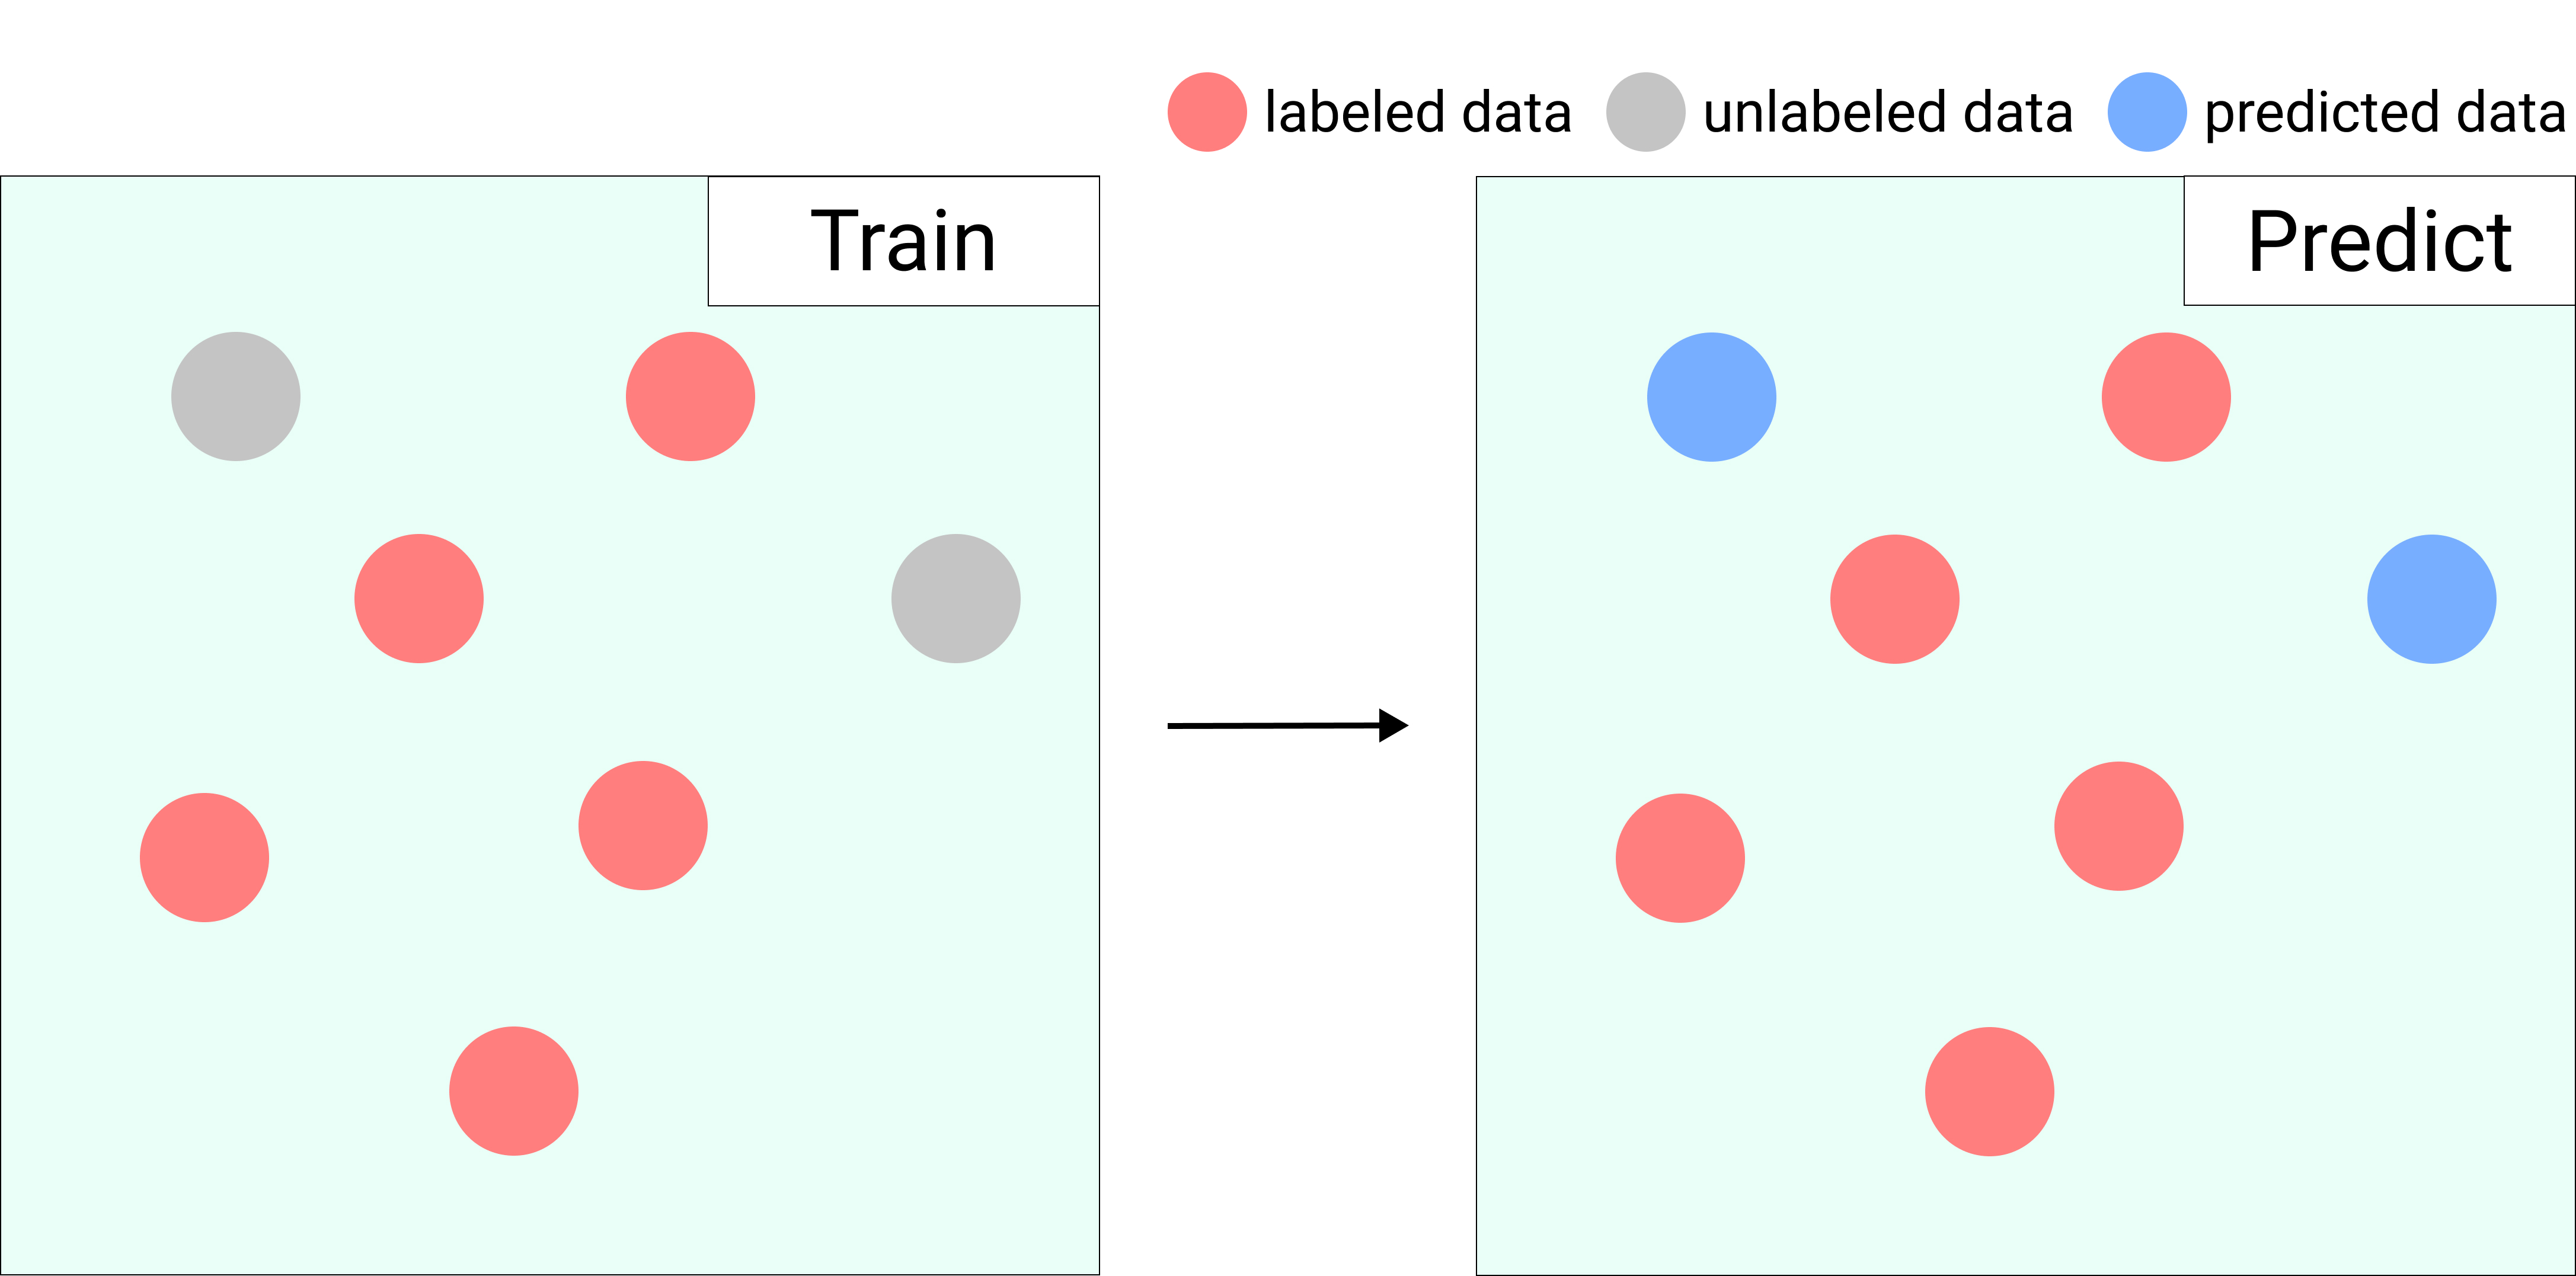
\includegraphics[width=\linewidth]
  {img/Transductive.jpg}
  \caption{トランスダクティブ学習}
  \label{fig:Transductive}
\end{figure}

それに比べて帰納学習とは, 学習時に存在しなかったデータに対しての推論を行う学習である. その様子を図 \ref{fig:Inductive} に示す.


\begin{figure}
  \centering
  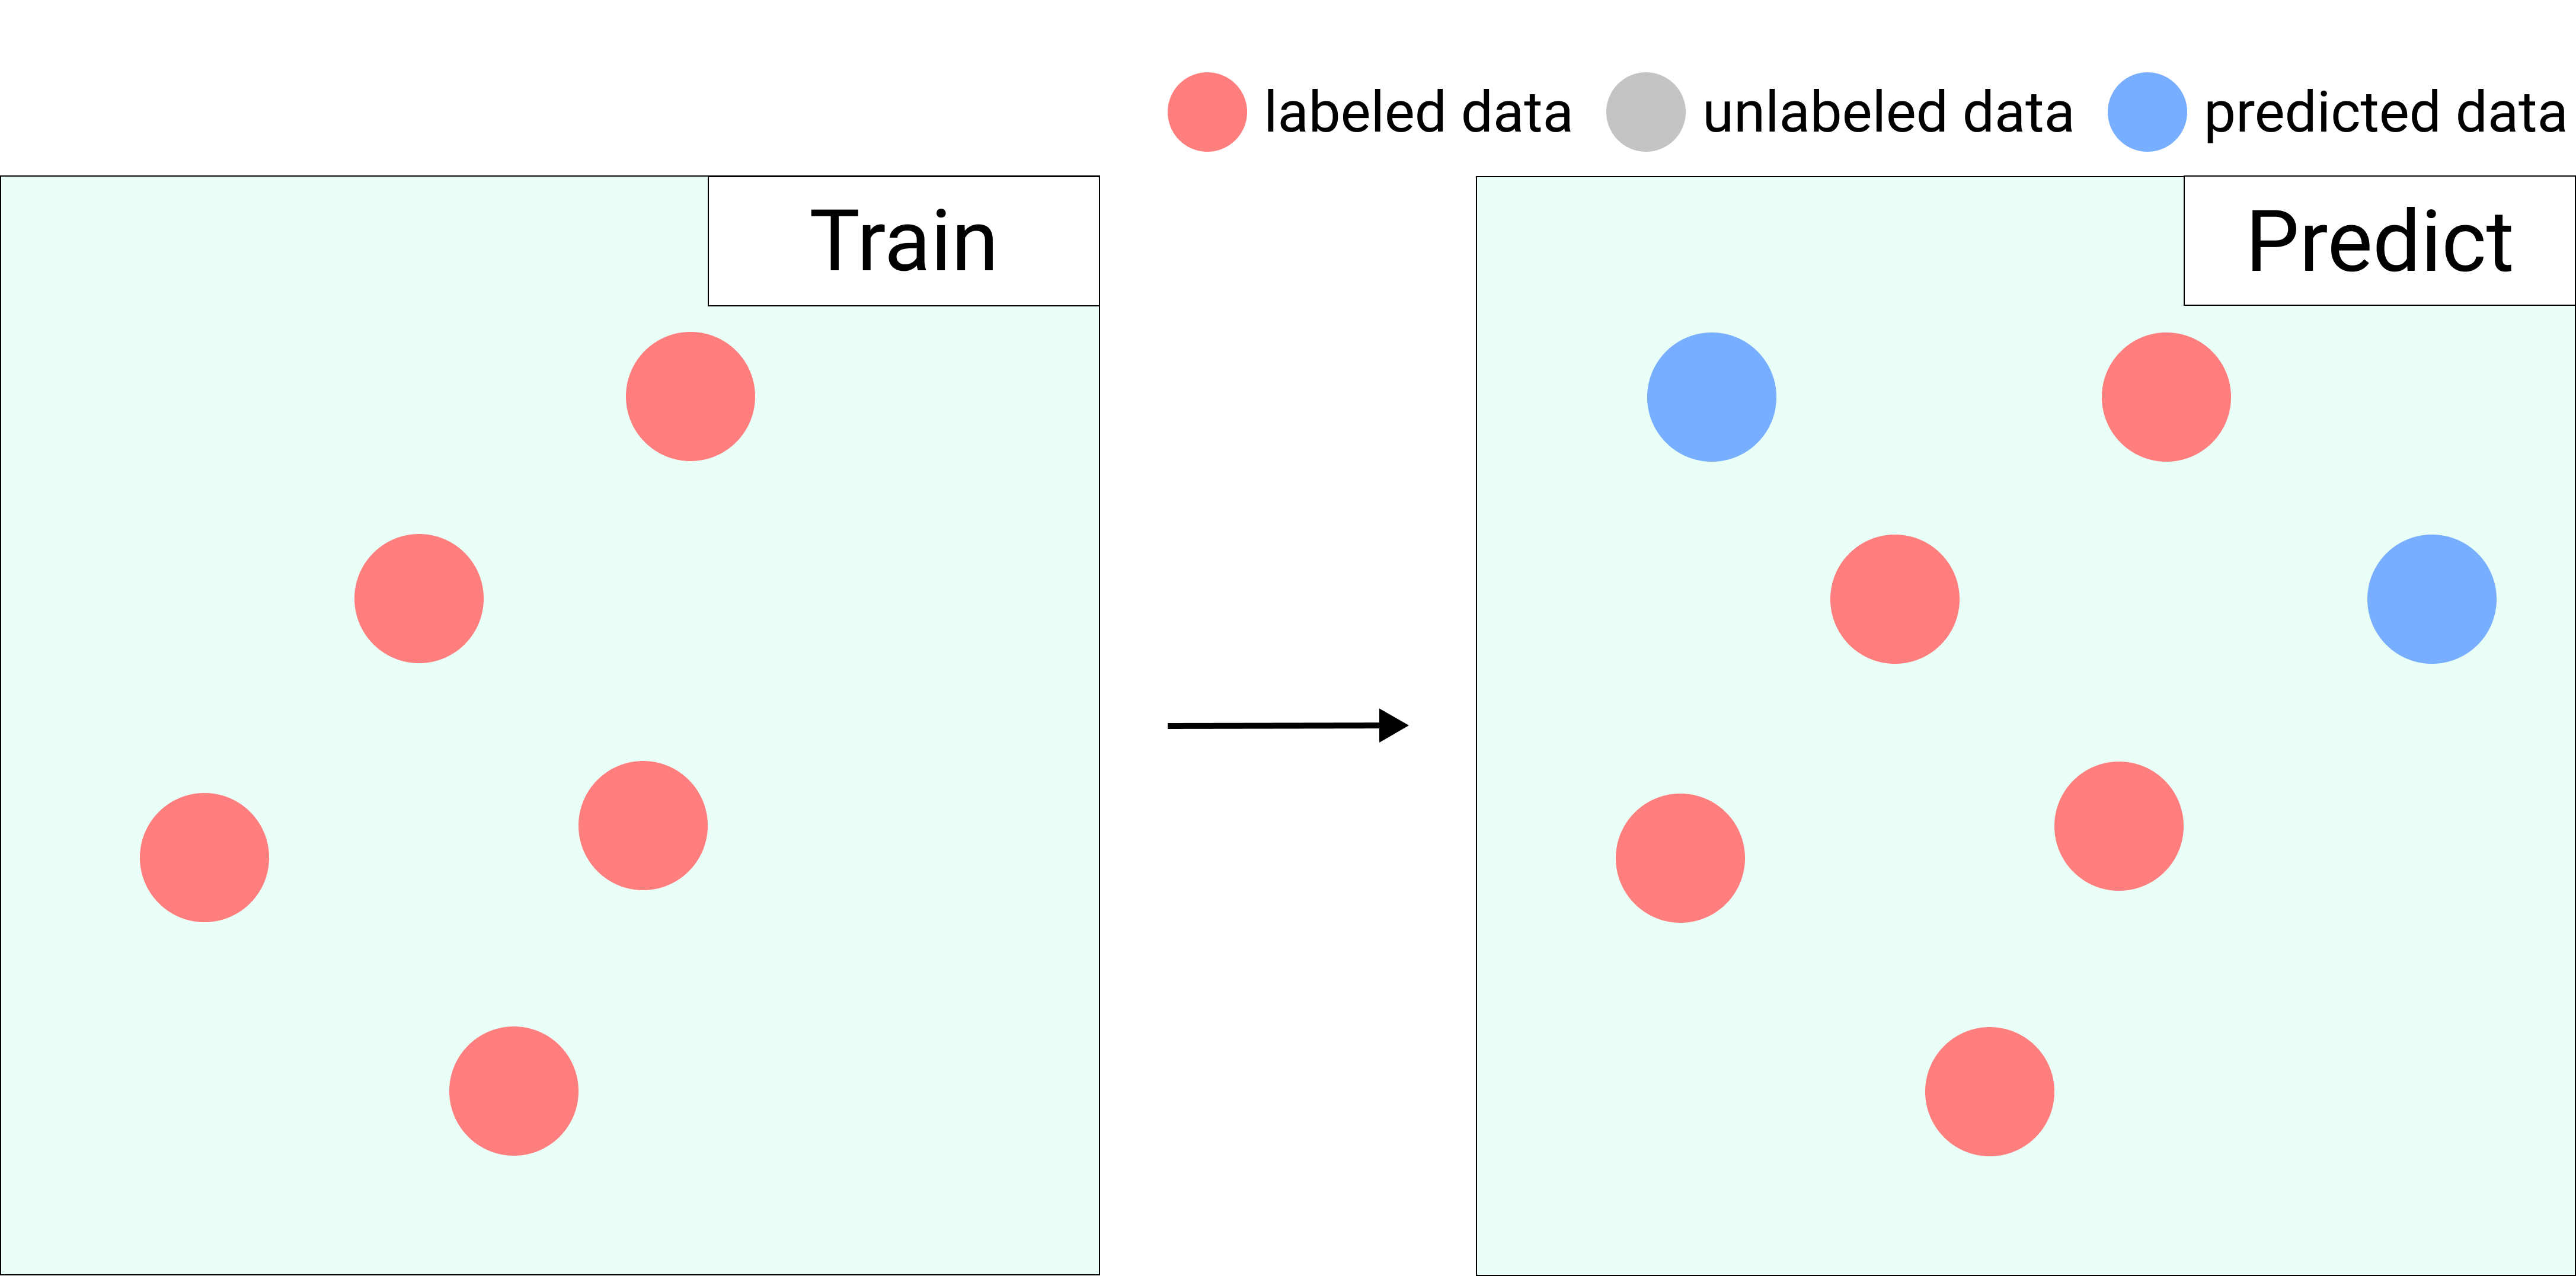
\includegraphics[width=\linewidth]
  {img/Inductive.jpg}
  \caption{帰納学習}
  \label{fig:Inductive}
\end{figure}


\subsection{fastText}
fastText\cite{bojanowski2017enriching}は Facebook AI Research によって開発された自然言語処理モデルである.このモデルを使用することで,単語埋め込みの生成やテキストの分類ができる.
本項では, Word2Vec で用いられている Skip-gram モデルについて説明し, その後, fastText で提案されたサブワードモデルについて説明する.
\subsubsection*{Skip-gram モデル}
Skip-gram モデルでは, サイズ W の単語の語彙が与えられ,単語はそのインデックス $w \in \{ 1,...,W \}$によって識別される場合, 各単語$w$のベクトル表現を学習することが目標となる.
分布仮説(周囲の単語によって単語の意味が形成されるという仮説)に基づき, 単語のベクトル表現はその文脈に現れる単語を予測して学習される.Skip-gram モデルでは式\ref{eq:fastLog}の対数尤度が最大になるように学習される.
\begin{equation}
  \label{eq:fastLog}
  \sum_{t=1}^{T} \sum_{c \in C_{t}} \log p(w_{c} | w_{t})
\end{equation}
ここで, T は与えられた文脈の長さ, $C_{t}$は注目単語$w_{t}$の周辺単語のインデックスの集合である.
注目単語と周辺単語のペアを実数にスコア付けする関数として$s(w_{t}, w_{c}) = \mathbf{u}_{w_{t}}^\mathsf{T}\mathbf{v}_{w_{c}}$(ここで,$\mathbf{u}_{w_{t}}, \mathbf{v}_{w_{c}}$は$w_{t}, w_{c}$に対応する単語ベクトル)が与えられるとする.
周辺単語が出現する確率$p(w_{c} | w_{t})$ の 1 つの選択肢として, 式\ref{eq:fastSoftmax}で示すソフトマックス関数が挙げられる.
\begin{equation}
  \label{eq:fastSoftmax}
  p(w_{c} | w_{t}) = \dfrac{e^{s(w_{t}, w_{c})}}{\sum_{j=1}^{W} e^{s(w_{t}, j)}}
\end{equation}
\par しかし, ソフトマックス関数を用いると計算量が大きくなる($W$は$10^5 〜 10^7$程度)という問題が存在する.
そのため,周辺単語の予測を,独立した二値分類問題の集合として構成する(Negative Sampling).
注目単語$w_{t}$に対して周辺単語$w_{c}$を正の例とし, 周辺単語以外の語彙からランダムに抽出した例を負の例とみなす.
その後,ロジスティック損失を用いて、式\ref{eq:loglike}に示す対数尤度を得る.

\begin{equation}
  \label{eq:loglike}
  \log (1 + e^{-s(w_{t}, w_{c})}) + \sum_{n \in \mathcal{N}_{t,c}} \log (1 + e^{s(w_{t}, n)})
\end{equation}
ここで, $\mathcal{N}_{t,c}$ が語彙からランダムに抽出した負の例の集合である.
最終的に, ロジスティク損失$l : x \mapsto \log(1+e^{-x})$とすると, Skip-gram モデルの目的は式\ref{eq:skipfin}を最小にすることである.
\begin{equation}
  \label{eq:skipfin}
  \sum_{t=1}^{T} \Biggl\lbrack \sum_{c \in C_{t}} l(s(w_{t}, w_{c})) + \sum_{n \in \mathcal{N}_{t,c}} l(-s(w_{t}, n))\Biggr\rbrack
\end{equation}

\par Skip-gram モデルでは各単語に個別のベクトル表現を用いており, 単語の内部構造は考慮していない.

\subsubsection*{サブワードモデル}
サブワードモデルでは, Skip-gram モデルで考慮されていなかった単語の内部構造を考慮するために, スコア付け関数を変更した.このモデルでは, 各単語の先頭と末尾に$<$と$>$を追加した,文字単位での$n$-gram を用いる. 例えば, \textsl{where}という単語に対して, $n=3$の場合の$n$-gram の集合は以下のようになる.
\centerline{$\{<$\textsl{wh, whe, her, ere, re}$>\}$}
このような, 文字単位での$n$-gram を利用したスコア付け関数は式\ref{eq:fastScore}で表される.
\begin{equation}
  \label{eq:fastScore}
  s(w,c) = \sum_{g\in \mathcal{G}_{w}} \mathbf{z}_{g}^\mathsf{T}\mathbf{v}_{c}
\end{equation}
ここで, $\mathcal{G}_{w}$は単語$w$の$n$-gram(実際には$n=3,4,5,6$のすべての$n$-gram)と$w$自身(\textsl{where}の例では$<$\textsl{where}$>$)の集合であり, $\mathbf{z}_{g}$は$n$-gram $g$のベクトル表現である.
\par サブワードモデルでは,スコア付け関数を変えたことによって単語の内部構造を考慮できるようになり, 出現頻度が低い語彙に対して, 信頼性の高い単語のベクトル表現を学習することができるようになった.
また, 単語の内部構造を考慮することにより, 未知語に対しても単語のベクトル表現を推論できるようになった.


\section{グラフニューラルネットワーク}\label{rel:GNN}
本節では, グラフニューラルネットワーク (GNN) に関する歴史や関連研究について述べる.
\subsection{GNNの歴史}
1997 年に Sperduti ら\cite{sperduti1997supervised}により, ニューラルネットワーク上で初めてグラフ構造が扱われた. この研究は初期の GNN の先駆的な研究となった.その後, Goriet ら\cite{gori2005anew},  Scarselli ら \cite{scarselli2009the} , Gallicchio ら \cite{gallicchio2010graph} により GNN に関する研究が行われてきた.
これらの研究は RNN のアーキテクチャを用いてグラフのノード埋め込みを学習することを目的としている(RecGNNs).
RecGNNs でのノードの更新は以下の 2 つの過程を繰り返す.
\begin{enumerate}
  \item 隣接ノード(+ノード自身)の状態を集約・解析 (メッセージパッシング)
  \item ノード自身の状態を更新
\end{enumerate}
周辺ノードの状態の集約はすべての層で同じ関数(かつ同じ重み)を用いて再帰的に行い, すべてのノードの状態が平衡状態になるまでノードの更新を続ける.
\par RecGNNs での第$l$層におけるノード$v$の出力$\mathbf{h}_{v}^{l}$は式\ref{eq:GNN}で表される.
\begin{equation}
  \label{eq:GNN}
  \mathbf{h}_{v}^{l}=\mathrm{Rec}(\mathbf{h}^{l-1}, \sum_{u \in \mathcal{N}(v)} W \mathbf{h}_{u}^{l})
\end{equation}
ここで, $\mathrm{Rec}$は RNN, LSTM などの再帰型ネットワーク, $\mathcal{N}(v)$はノード$v$の隣接ノードの集合である.
RecGNNs には計算コストが非常に高いという問題がある.
RecGNNs のメッセージパッシングの概念は, GCN に受け継がれている.
\subsection{Graph Convolutional Network}
Graph Convolutional Network (GCN) \cite{kipf2017semi} は,CNN のような畳み込み演算を GNN に適用したモデルである.1 層の GCN を用いるとそれぞれのノードが隣接するノードの情報を畳み込むという特徴がある. GCN は RecGNNs とは異なり, 層ごとに異なる重みを用いる.
隣接行列 $A$ と特徴行列 $X$ を GCN に与える入力とすると,GCN の第$l$層における出力$\mathbf{h}^{l}$は式\ref{eq:GCN}で表される.
\begin{equation}
  \label{eq:GCN}
  \mathbf{h}^{l}=f(\tilde{D}^{-\frac{1}{2}}\tilde{A}\tilde{D}^{-\frac{1}{2}}\mathbf{h}^{l-1}W_{1}^{(l-1)})
\end{equation}
ここで,$\tilde{A} = A + I_{N}$はノード自身へのエッジを追加した無向グラフの隣接行列であり,$I_N$は単位行列である.
$\tilde{D}_{ii} = \sum_{j} \tilde{A}_{ij}$であり,$W_{1}^{(l)}$は層に応じた学習可能な重み行列,$f(\cdot)$は$ReLU(\cdot) = \max (0, \cdot)$のような活性化関数である.
また,$H^{(0)}=X$となる.\par
GCN は層の数を増やしすぎると,全てのノードの埋め込みが同じ値に収束してしまい,性能が低下することがわかっている.

\subsection{GraphSAGE}
GraphSAGE は GCN を拡張したものであり, 帰納学習を行うことができるモデルである. GCN との違いとして, GraphSAGE では近傍ノードを抽出し, それを集約するための aggregate 関数を学習を学習する.GraphSAGE での前方伝播では, まずノードの近傍ノードを抽出し, サブグラフを作成する.
その後, 近傍ごとに異なる aggregate 関数を用いて, サブグラフ内のノードから特徴量を集約する.
最終的に集約した特徴量を元にラベルの推論を行う.前方伝播の過程を図\ref{fig:SAGE}に示す.

\begin{figure}
  \centering
  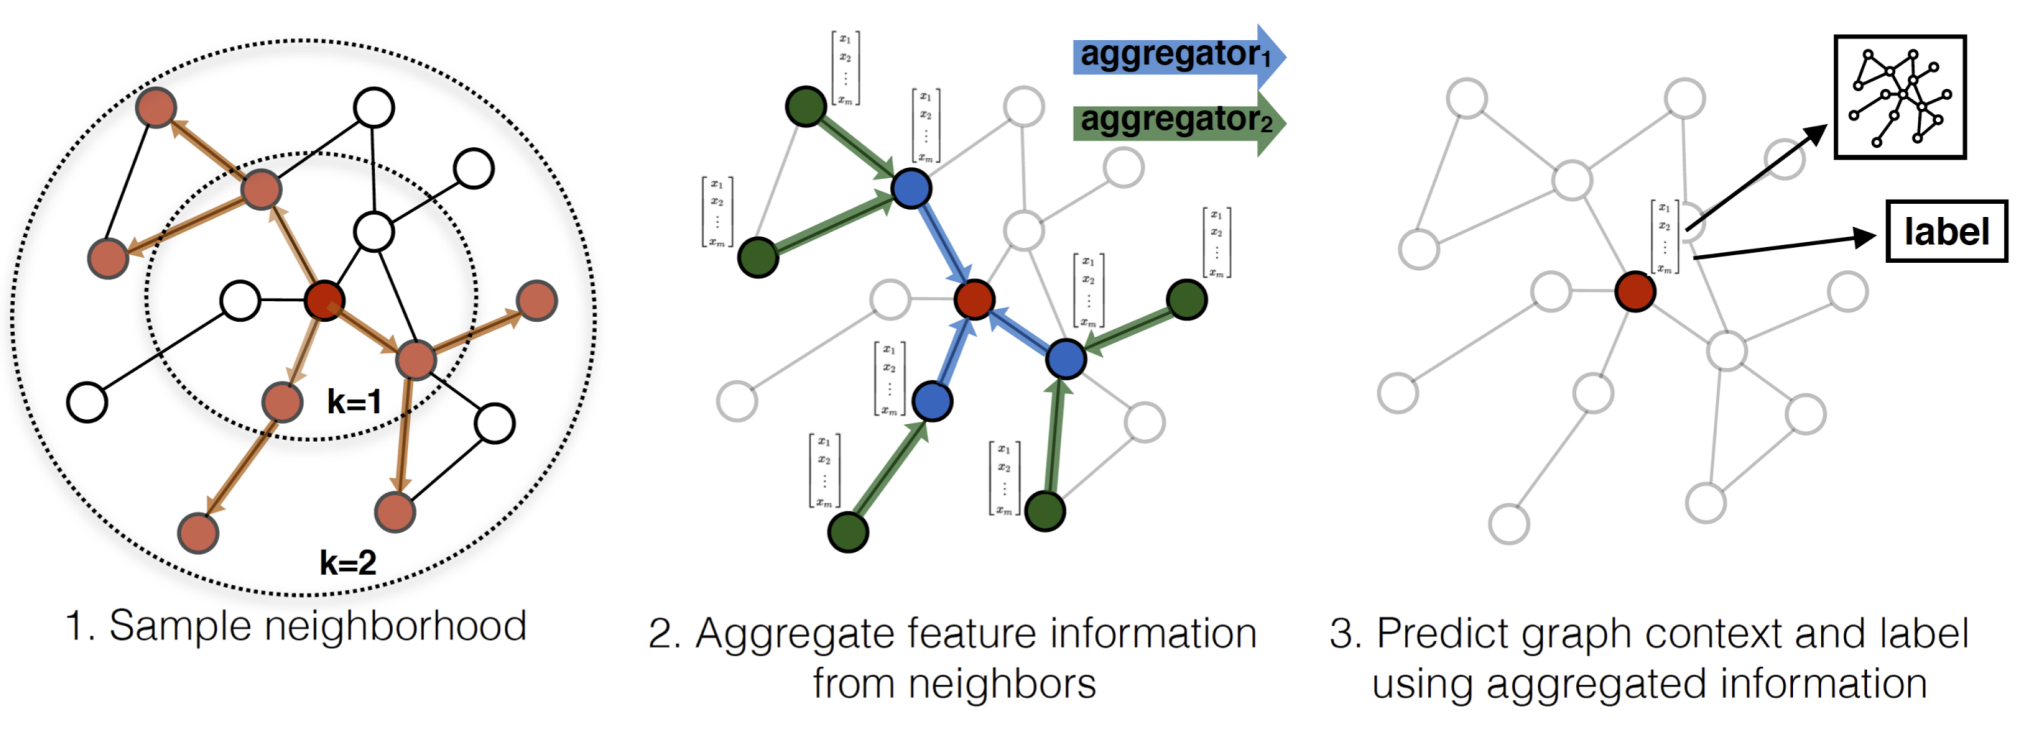
\includegraphics[width=\linewidth]
  {img/GraphSAGE.png}
  \caption{GraphSAGEの前方伝播 (\cite{hamilton2017inductive}より引用)}
  \label{fig:SAGE}
\end{figure}

aggregate 関数のアーキテクチャには 3 種類が存在する.
\subsubsection{Mean aggregator}
Mean aggregator を用いた場合, ノード$v$に対する GraphSAGE の第$l$層の出力$\mathbf{h}_{v}^{l}$は式\ref{eq:MeanAgg}で表される.
\begin{equation}
  \label{eq:MeanAgg}
  \mathbf{h}_{v}^{l} \leftarrow \sigma(\mathbf{W_{2}} \cdot \mathrm{MEAN} (\{ \mathbf{h}_{v}^{l-1}\} \cup \{ \mathbf{h}_{u}^{l-1} , \forall u \in \mathcal{N}(v) \}))
\end{equation}
ここで, $\mathbf{h}_{v}^{l}$は第$l$層でのノード$v$の埋め込みであり, $\mathbf{W_{2}}$は学習可能な重み行列, $\mathcal{N}(v)$はノード$v$の近傍ノード郡である.
このアーキテクチャは GCN と同様の処理を 帰納学習に対応させたものである.

\subsubsection{LSTM aggregator}
LSTM aggregator は, LSTM アーキテクチャに基づくより複雑な aggregator である. Mean aggregator に比べて, LSTM aggregator は表現力に優れている. しかし, LSTM は入力を逐次的に処理するため, ノードの入力順に応じて結果が変化する. そのため, ノードの近傍を不規則に並び替えることで, 非順序集合で LSTM を動作させた.

\subsubsection{Pooling aggregator}
Pooling aggregator は, 近傍ノードを全結合層に与え, その結果の中で最大となるものを選択する.これは, 式\ref{eq:PoolAgg}で表される.
\begin{equation}
  \label{eq:PoolAgg}
  \mathrm{AGGREGATE}_{k}^{\mathrm{pool}} = \max(\{ \sigma ( \mathbf{W_{2}}_{pool} \mathbf{h}_{u_{i}}^{k} + \mathbf{b} ), \forall u_{i} \in \mathcal{N}(v) \})
\end{equation}
ここで, $\sigma$ は非線形の活性化関数であり, $\mathbf{b}$はバイアスである.

\subsection{SimGNN}
SimGNN\cite{bai2019simgnn}は GNN を用いて近似的に Graph Edit Distance(GED)を求めるモデルである.グラフの入力ノードにはラベルが割り振られており,ノードの特徴量はラベルの One-Hot ベクトルとなる.
この手法では,入力グラフを複数層の GCN に与えることでノードレベルの埋め込みを生成した後,以下に示すアテンションモジュールを元にグラフレベルの埋め込みを生成する.
それらの非線形の変換をし, global graph context $c \in \mathbb{R}^{D}$を得る.
\begin{equation}c = \tanh (\frac{1}{N}W_{3}{\displaystyle \sum_{n=1}^{N}} u_{n})\end{equation}
ここで,$u_{n} \in \mathbb{R}^{D}$は入力ノード$n$の埋め込み,$D$はノードの埋め込みの次元,$W_{3} \in \mathbb{R}^{D \times D}$は学習可能な重み行列である.
$c$は重み行列を学習することで,グラフの全体的な構造及び特徴量を表すことができ,これに基づいて各ノードの重要度を計算することが可能となる.\par
ノード$n$に対しての重要度$a_{n}$の計算は,ノード$n$の埋め込み$u_{n}$と$c$の内積を計算した後,シグモイド関数$\sigma(x) = \frac{1}{1+exp(-x)}$を用いることで,重要度$a_{n}$を$(0,1)$の範囲に収める.
ここではグラフサイズを埋め込みに反映するため,全体の重要度を正規化しない.
重要度を計算した後,グラフレベルの埋め込み$h \in \mathbb{R}^{D}$を重み付きのノードの埋め込みの総和$h = \sum_{n=1}^{N}a_{n}u_{n}$で計算する.
アテンションモジュールについてまとめると式\ref{eq:Att}になる.
\begin{equation}
  \label{eq:Att}
  h = \sum_{n=1}^{N}\sigma(u_{n}^\mathsf{T}c)u_{n}= \sum_{n=1}^{N}\sigma(u_{n}^\mathsf{T} \tanh (\frac{1}{N}W_{3}\sum_{m=1}^{N}u_{m}))u_{n}
\end{equation}
AttentionModule から 2 つのグラフの埋め込み$h_{i} \in \mathbb{R}^{D}, h_{j} \in \mathbb{R}^{D}$が与えられた後,
それらの関係をモデル化するために,式\ref{eq:NTN} で表されるニューラルテンソルネットワークを用いる.
\begin{equation}
  \label{eq:NTN}
  g(h_{i}, h_{j})=f(h_{i}^\mathsf{T}W_{4}^{[1:K]}h_{j} + V \begin{bmatrix} h_{i}\\h_{j} \end{bmatrix} + b)
\end{equation}

ここで,$W_{4}^{[1:K]} \in R^{D \times D \times K}$は重み行列,$\begin{bmatrix} $ $ \end{bmatrix}$は結合操作,$V \in \mathbb{R}^{K\times2D}$は重みベクトル.
$b \in \mathbb{R}^{K}$はバイアスベクトル,$f(\cdot)$は$ReLU(\cdot) = \max (0, \cdot)$のような活性化関数である.
$K$は K は各グラフ埋め込みペアに対してモデルが生成する類似度の数を制御するハイパーパラメータである.\par


\subsection{Self-Attention Graph Pooling (SAGPool)}
Self-Attention Graph Pooling (SAGPool) \cite{lee2019self} はグラフプーリング手法の 1 つである. SAGPool を用いることで Self-Attention に基づいたノードの削減を行うことができる. この手法では, ノードの重要度は式\ref{eq:SAScore}で示される.
\begin{equation}
  \label{eq:SAScore}
  Z = \sigma (\tilde{D}^{-\frac{1}{2}}\tilde{A}\tilde{D}^{-\frac{1}{2}}X\Theta_{att})
\end{equation}
ここで, $\tilde{A} = A + I_{N}$はノード自身へのエッジを追加した無向グラフの隣接行列であり,$I_N$は単位行列である.
$\tilde{D}_{ii} = \sum_{j} \tilde{A}_{ij}$であり$\Theta_{att}$は SAGPool 層のパラメータである.
GCN を用いることで, グラフの特徴と構造情報の両方に基づいた重要度を得ることができる.
ノードの重要度を元に, Gao ら\cite{gao2019proceedings} によるノード選択方法を行うことで, 上位$\lceil kN \rceil$個のノードを保持する.ここで,$k \in (0,1)$はプーリングの割合である. 式\ref{eq:topk}はノード選択法を表す.
\begin{equation}
  \label{eq:topk}
  \mathrm{idx} = \textrm{top-rank}(Z, \lceil kN \rceil ), Z_{mask} = Z_{\mathrm{idx}}
\end{equation}
ここで, $\textrm{top-rank}$ は上位$\lceil kN \rceil$個のノードを返し, $\cdot_{\mathrm{idx}}$は$\mathrm{idx}$が示すノードのみの重要度である.
最終的に, 式\ref{eq:SAGPool}に表すように, 上位$\lceil kN \rceil$個のノードのみのグラフを作成する.
\begin{equation}
  \label{eq:SAGPool}
  X' = X_{\mathrm{idx},:}, X_{out} = X' \odot Z_{mask}, A_{out} = A_{\mathrm{idx,idx}}
\end{equation}
ここで, $X_{\mathrm{idx},:}$は$\mathrm{idx}$が示すノードの特徴量行列であり, $\odot$ はアダマール積 (要素ごとの積) であり, $A_{\mathrm{idx,idx}}$は$\mathrm{idx}$が示すノードの隣接行列である.

% 本原稿用の条件マクロ
% これ以降は削除しちゃダメ
\expandafter\ifx\csname MasterFile\endcsname\relax
\def\MasterFile{本原稿です}

% 参考文献
%% 本原稿用の条件マクロ
%章ごとにコンパイルできるようにするための設定.
%このマクロが定義されていない場合,チャプター内は個別のTEXソースとして扱われる.
\expandafter\ifx\csname MasterFile\endcsname\relax
\documentclass[a4j,12pt]{thesis} % 修論・卒論など (ページが右端にでる)   
\usepackage{mysettings}
\usepackage{url}

\begin{document}

\setlength{\baselineskip}{1.95zw}
\setlength{\textheight}{30\baselineskip}
\backmatter

\fi
% これより上は削除しちゃダメ
% 本原稿用の条件マクロここまで

%参考文献

\bibliographystyle{junsrt}
\bibliography{thesisB}

\clearpage


% 本原稿用の条件マクロ
% これ以降は削除しちゃダメ
\expandafter\ifx\csname MasterFile\endcsname\relax
\def\MasterFile{本原稿です}
\end{document}
\fi
% 本原稿用の条件マクロここまで


\bibliographystyle{junsrt}
\bibliography{thesisB}

\end{document}
\fi
% 本原稿用の条件マクロここまで
 
% 本原稿用の条件マクロ
%章ごとにコンパイルできるようにするための設定.
%このマクロが定義されていない場合,チャプター内は個別のTEXソースとして扱われる.
\expandafter\ifx\csname MasterFile\endcsname\relax
\documentclass[a4j,twoside,12pt, dvipdfmx]{thesis} % 修論・卒論など (ページが右端にでる) 
\usepackage{amsmath, amssymb}
\usepackage{mysettings}
\usepackage{graphicx}
\usepackage{color}
\usepackage{comment}

\begin{document}

\addtocounter{chapter}{+2}

\setlength{\baselineskip}{1.95zw}
\setlength{\textheight}{30\baselineskip}
\mainmatter

\fi
% これより上は削除しちゃダメ
% 本原稿用の条件マクロここまで
%
%\newcommand{\argmax}{\mathop{\rm arg~max}\limits}
\renewcommand\thefootnote{\arabic{footnote})}
\def\vector#1{\mbox{\boldmath $#1$}}

\chapter{提案手法}\label{meth}
% ここに本文
本章では,提案手法について説明する.本研究は大きく分けて以下の 4 つに分類される.
\begin{enumerate}
  \item 文からのグラフ作成
  \item ノードの特徴量畳込み
  \item グラフを表現する埋め込み生成
  \item グラフ間の類似度の評価
\end{enumerate}
それぞれの方法について 2 種類の手法を採用し, 計 16 種類の手法で比較を行った. \par
モデルの概要を図\ref{fig:ModelFlow}に示す.
\begin{figure}
  \centering
  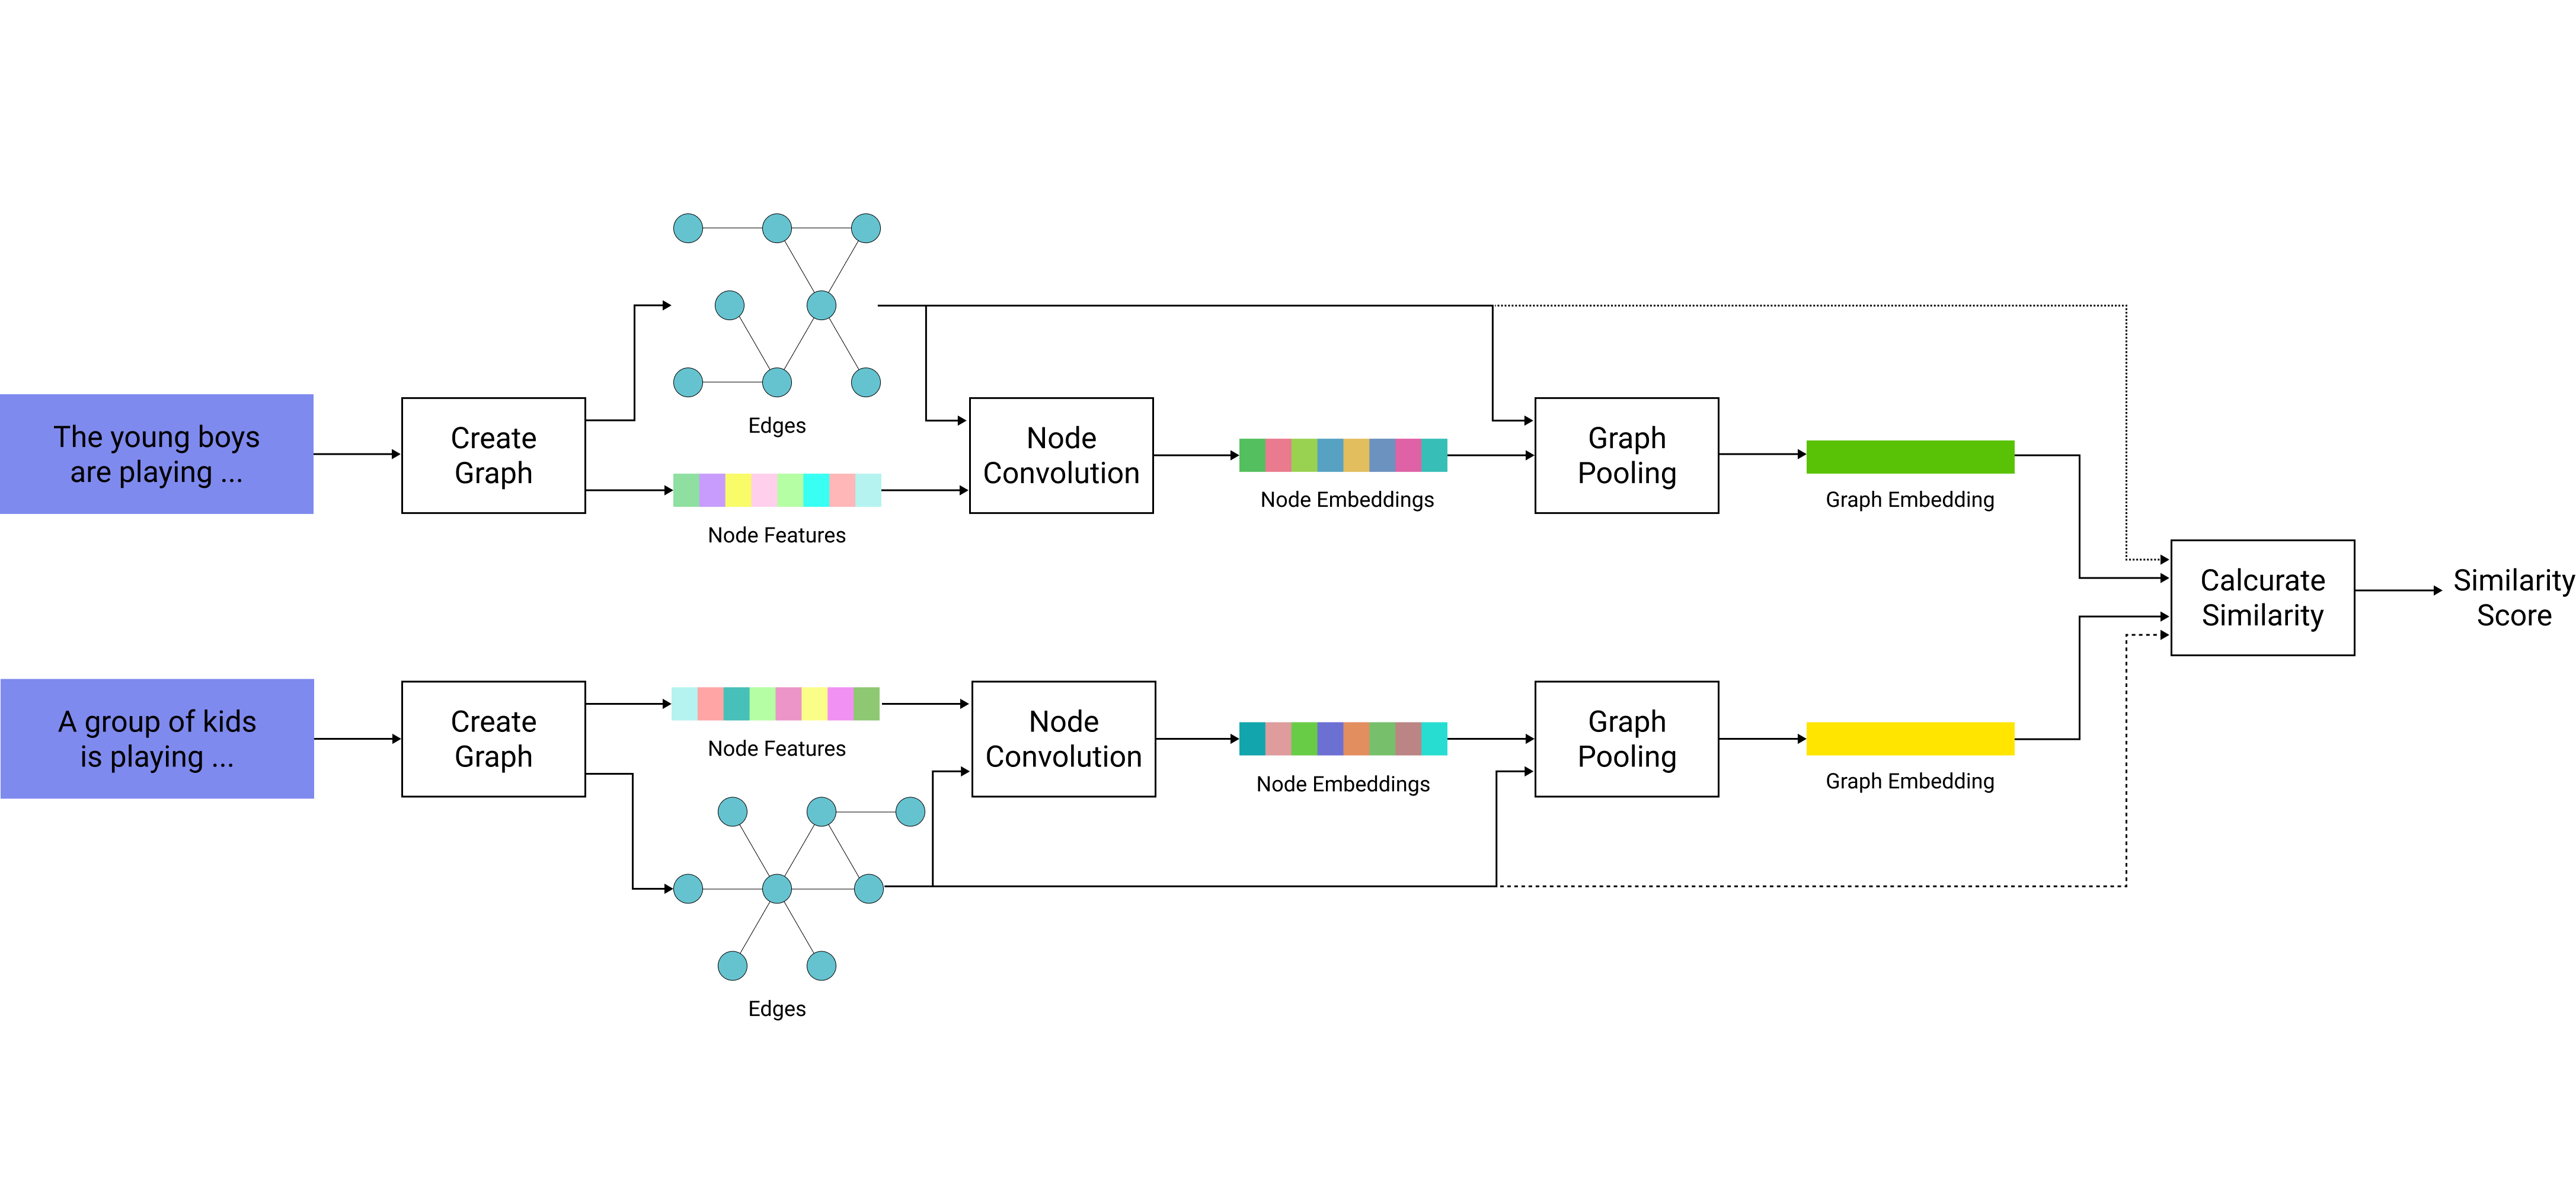
\includegraphics[width=\linewidth]
  {img/ModelFlow.jpg}
  \caption{モデルの概要}
  \label{fig:ModelFlow}
\end{figure}

\ref{meth:createGraph}節では文からのグラフ作成,\ref{meth:convNode}節ではノード畳込み \ref{meth:createEmbedding}節ではグラフを表現する埋め込み生成, \ref{meth:calculateSimilarity}節ではグラフ間の類似度計算について述べる.

\section{文からのグラフ作成}\label{meth:createGraph}
本節では,文からのグラフ生成手法について説明する.\
グラフの生成について,以下の2つを行う.
\begin{enumerate}
  \item ノード生成
  \item エッジ生成
\end{enumerate}
また, 本研究では以下の2通りのエッジ生成方法を元に, 2 種類のグラフを生成し実験した.
\begin{enumerate}
  \item 依存関係に基づくエッジ生成
  \item 依存関係と隣接関係に基づくエッジ生成
\end{enumerate}

\subsection{ノード生成}\label{meth:createNode}
文からのグラフの生成において,各ノードはそれぞれの単語とし,その単語のレンマの埋め込みを取得し,ノードの特徴量とした.

\subsection{エッジ生成}\label{meth:createEdge}
構文情報には単語間の依存情報や隣接関係などが存在する. そこで本研究では, 依存関係に基づくエッジの生成方法と, それに加えて隣接関係も追加したエッジの生成方法の 2 つを採用した.
隣接関係のみに基づくエッジの生成を行わなかった理由としては, 隣接関係のみだとグラフ構造が鎖状になってしまうためである.
\subsubsection*{依存関係に基づくエッジ生成}
各エッジの生成には Universal Dependencies に基づく構文解析を行い,単語間に依存関係があれば双方向にエッジを作成し,無向グラフを生成した.

\subsubsection*{依存関係と隣接関係に基づくエッジ生成}
依存関係に基づくエッジ生成に加えて, 単語間に隣接関係があれば双方向エッジを作成し,無向グラフを生成した.

\section{ノードの特徴量畳込み}\label{meth:convNode}
本節では, ノードの特徴量畳込み手法について説明する.
ノードの特徴量畳み込みでは 2 通りの方法を採用した.
\subsection{Graph Convolutional Network (GCN)}
この方法では,ノードの畳み込みに Kipf ら\cite{kipf2017semi}と同様の Graph Convolutional Network (GCN) を用いた.
この方法は SimGNN\cite{bai2019simgnn}でも用いられている.
GCN の第$l$層における出力は式\ref{eq:methGCN}で表される.
\begin{equation}
  \label{eq:methGCN}
  H^{(l)}=f(\tilde{D}^{-\frac{1}{2}}\tilde{A}\tilde{D}^{-\frac{1}{2}}H^{(l-1)}W_{1}^{(l-1)})
\end{equation}
ここで,$\tilde{A} = A + I_{N}$はノード自身へのエッジを追加した無向グラフの隣接行列であり,$I_N$は単位行列である.
$\tilde{D}_{ii} = \sum_{j} \tilde{A}_{ij}$であり,$W_{1}^{(l)}$は層に応じた学習可能な重み行列,$f(\cdot)$は$ReLU(\cdot) = \max (0, \cdot)$のような活性化関数である.
また,$H^{(0)}=X$となる.

\subsubsection{GraphSAGE}
この方法では, ノードの畳み込みに GraphSAGE\cite{hamilton2017inductive} (SAGE) を用いた.
本手法を採用した背景は, 近傍ノードをサンプリングして学習する GraphSAGE を用いることで, グラフサイズの影響を減らして効果的に特徴量の畳み込みができるだろうと言う直感に基づいている.
aggregator には, MeanAggregator を用いる.
Mean aggregator を用いた場合, ノード$v$に対する GraphSAGE の第$l$層の出力は式\ref{eq:methGraphSAGE}で表される.
\begin{equation}
  \label{eq:methGraphSAGE}
  h_{v}^{l} \leftarrow \sigma(\mathbf{W_{2}} \cdot \mathrm{MEAN} (\{ \mathbf{h}_{v}^{l-1}\} \cup \{ \mathbf{h}_{u}^{l-1} , \forall u \in \mathcal{N}(v) \}))
\end{equation}
ここで, $\mathbf{h}_{v}^{l}$は第$l$層でのノード$v$の埋め込みであり, $\mathbf{W_{2}}$は学習可能な重み行列, $\mathcal{N}(v)$はノード$v$の近傍ノード郡である.

\section{グラフを表現する埋め込み生成}\label{meth:createEmbedding}
本節では,グラフを表現する埋め込み生成手法について説明する.
グラフを表現する埋め込み生成では 2 通りの方法を採用した.
これらの方法では, 前節の方法で得られたノードレベルの埋め込みを元にグラフを表現する埋め込みを生成する.

\subsection{アテンションモジュール}
この方法は SimGNN で用いられているアテンションモジュール (Att) と同様のものである.
アテンションモジュールから出力される, グラフを表現する埋め込み$h$は以下の式で表される.
\begin{equation}
  h = \sum_{n=1}^{N}\sigma(u_{n}^\mathsf{T}c)u_{n}= \sum_{n=1}^{N}\sigma(u_{n}^\mathsf{T} \tanh (\frac{1}{N}W_{2}\sum_{m=1}^{N}u_{m}))u_{n}
\end{equation}
ここで, $u_{n}$ はノード$n$の埋め込み, $\sigma$ はシグモイド関数, $N$はノード数, $W_{2}$は学習可能な重み行列である.

\subsection{SAGPool}
この方法では, グラフを表現する埋め込み生成に Self-Attention Graph Pooling (SAGPool) \cite{lee2019self} を用いた.
本手法を採用した背景は, 畳み込みを行った後に最も周辺ノードの情報を集めることができたノードはグラフ全体を表しているのではないかという直感に基づいている.
SAGPool では, 各ノードの重要度を式\ref{eq:methAtt} で算出し, 重要度が最も高いノードの表現からグラフを表現する埋め込みを取得する.
\begin{equation}
  \label{eq:methAtt}
  Z = \sigma (\tilde{D}^{-\frac{1}{2}}\tilde{A}\tilde{D}^{-\frac{1}{2}}X\Theta_{att})
\end{equation}
ここで, $\tilde{A} = A + I_{N}$はノード自身へのエッジを追加した無向グラフの隣接行列であり,$I_N$は単位行列である.
$\tilde{D}_{ii} = \sum_{j} \tilde{A}_{ij}$であり$\Theta_{att}$は SAGPool 層のパラメータである.

\section{グラフ間の類似度計算}\label{meth:calculateSimilarity}
本節では, グラフ間の類似度計算手法について説明する.
グラフ間の類似度計算では 2 通りの方法を採用した.
これらの方法では, 前節の方法で得られたグラフを表現する埋め込みから類似度を計算する.

\subsection{ニューラルテンソルネットワーク}
この方法は SimGNN で用いられている ニューラルテンソルネットワーク (NTN) と同様のものである.
2 つのグラフの埋め込み$h_{i}$, $h_{j}$を ニューラルテンソルネットワーク に与えた出力は式\ref{eq:NTN}である.
\begin{equation} \label{eq:NTN} g(h_{i}, h_{j})=f(h_{i}^\mathsf{T}W_{3}^{[1:K]}h_{j} + V \begin{bmatrix} h_{i}\\h_{j} \end{bmatrix} + b)\end{equation}
を用いる.
ここで,$W_{3}^{[1:K]} \in R^{D \times D \times K}$は重み行列,$\begin{bmatrix} $ $ \end{bmatrix}$は結合操作,$V \in \mathbb{R}^{K\times2D}$は重みベクトル.
$b \in \mathbb{R}^{K}$はバイアスベクトル, $f(\cdot)$は$ReLU(\cdot) = \max (0, \cdot)$のような活性化関数である.得られた出力を 2 層の全結合層に与えることで, 最終的な類似度を得る.

\subsection{コサイン類似度}
この方法はコサイン類似度 (cos) を用いてグラフ間の類似度計算を行うものである.
本手法を採用した理由は, ベクトル間の類似度を求めるのに一般的に用いられているコサイン類似度を利用することで, ニューラルテンソルネットワークの有効性を検証するためである.
2 つのグラフの埋め込み$h_{i}$, $h_{j}$のコサイン類似度は,式\ref{eq:cos}で表される.
\begin{equation}
  \label{eq:cos}
  \cos(h_{i}, h_{j}) = \dfrac{h_{i} \cdot h_{j}}{|h_{i} | | h_{j}|}
\end{equation}

% 本原稿用の条件マクロ
% これ以降は削除しちゃダメ
\expandafter\ifx\csname MasterFile\endcsname\relax
\def\MasterFile{本原稿です}

% 参考文献
%% 本原稿用の条件マクロ
%章ごとにコンパイルできるようにするための設定.
%このマクロが定義されていない場合,チャプター内は個別のTEXソースとして扱われる.
\expandafter\ifx\csname MasterFile\endcsname\relax
\documentclass[a4j,12pt]{thesis} % 修論・卒論など (ページが右端にでる)   
\usepackage{mysettings}
\usepackage{url}

\begin{document}

\setlength{\baselineskip}{1.95zw}
\setlength{\textheight}{30\baselineskip}
\backmatter

\fi
% これより上は削除しちゃダメ
% 本原稿用の条件マクロここまで

%参考文献

\bibliographystyle{junsrt}
\bibliography{thesisB}

\clearpage


% 本原稿用の条件マクロ
% これ以降は削除しちゃダメ
\expandafter\ifx\csname MasterFile\endcsname\relax
\def\MasterFile{本原稿です}
\end{document}
\fi
% 本原稿用の条件マクロここまで


\bibliographystyle{junsrt}
\bibliography{thesisB}

\end{document}
\fi
% 本原稿用の条件マクロここまで
			% 提案手法
% 本原稿用の条件マクロ
%章ごとにコンパイルできるようにするための設定.
%このマクロが定義されていない場合,チャプタ内は個別のTEXソースとして扱われる.
\expandafter\ifx\csname MasterFile\endcsname\relax
\documentclass[a4j,twoside,12pt]{thesis} % 修論・卒論など (ページが右端にでる)   

\usepackage{mysettings}
\usepackage{url}
\usepackage{bm}
\usepackage[table,xcdraw]{xcolor}
\usepackage{multirow}
\usepackage[subrefformat=parens]{subcaption}
\usepackage[dvipdfmx]{graphicx}
\usepackage{tabularx}
\usepackage{diagbox} 

\newcommand{\bhline}[1]{\noalign{\hrule height #1}}  
\newcommand{\bvline}[1]{\vrule width #1}  
\newcolumntype{Y}{&gt;{\centering\arraybackslash}X} %中央揃え

\captionsetup{labelsep = quad}
\captionsetup{subrefformat = parens}
\captionsetup{compatibility=false}
\begin{document}

\addtocounter{chapter}{+3}

\setlength{\baselineskip}{1.95zw}
\setlength{\textheight}{30\baselineskip}
\mainmatter

\fi
% これより上は削除しちゃダメ
% 本原稿用の条件マクロここまで
\renewcommand\thefootnote{\arabic{footnote})}


\chapter{実験}\label{exper}
% ここに本文
\section{実験環境}
実験環境は以下のとおりである.
\subsection*{ハードウェア}
\begin{itemize}
  \item CPU: AMD Ryzen9 5900X(12コア24スレッド)
  \item メモリ: 32GB
  \item GPU: RTX 3090
  \item GPU メモリ: 24GB
\end{itemize}
\subsection*{ソフトウェア}
\begin{itemize}
  \item OS: Ubuntu 20.04
  \item CUDA: 11.2
  \item cuDNN: 8.1
  \item PyTorch: 1.10.1
\end{itemize}

\section{データセット}
実験には Sentences Involving Compositional Knowledge (SICK) データセットと Semantic Textual Similarity benchmark (STS-b) データセットを用いた.
それぞれのデータセットには文のペアとその類似度が 0-5 の範囲で含まれている.それぞれのデータセットの詳細は以下の表\ref{table:dataset}の通りである.
\begin{table}
  \caption{データセットの詳細}
  \label{table:dataset}
  \centering
  \begin{tabular}{l|rrrr}
    \bhline{1pt}
          & \multicolumn{1}{c}{train} & \multicolumn{1}{c}{test} & \multicolumn{1}{c}{validation} & \multicolumn{1}{c}{total} \\
    \hline
    SICK  & 4,439                     & 4,906                    & 495                            & 9,840                     \\
    STS-b & 5,749                     & 1,379                    & 1,500                          & 8,628                     \\
    \bhline{1pt}
  \end{tabular}
\end{table}

\section{グラフの作成}
この節では, グラフの作成について述べる.

\subsection{ノード生成}
各ノードはそれぞれの単語とし, ノードを生成した.
各ノードの特徴量は,対応する単語のレンマをもとに, 事前学習済み fastText\cite{bojanowski2017enriching} モデルから得られるものとした.
ここで, 事前学習済みモデルには Common Crawl データセットでの事前学習済みモデルを利用した.
本研究では, 未知語に対応するために Word2Vec ではなく fastText を利用した.

\subsection{エッジ生成}
エッジの生成方法では,2 種類の方法について以下のように実験を行った.
\subsubsection{依存関係に基づくエッジ生成}
依存関係に基づくエッジ生成には, Stanza\cite{qi2020stanza} ライブラリを利用した Universal Dependencies に基づく係り受け解析を用いた.
係り受け解析の結果から, 単語間に依存関係が存在した場合に双方向エッジを作成した.

\subsubsection{依存関係と隣接関係に基づくエッジ生成}
依存関係と隣接関係に基づくエッジ生成には, 依存関係に基づくエッジに加えて, 単語間に隣接関係があれば双方向エッジを作成した.

\section{ハイパーパラメータ}
この節ではモデルのハイパーパラメータについて説明する.
GCN \cite{kipf2017semi} ( GraphSAGE \cite{hamilton2017inductive} ) の層数は 3 層とし, GCN の第 1 層, 第 2 層, 第 3 層の出力次元はそれぞれ 128, 64, 32 とした. また, NTN 層では $K=16$ とした.

\section{評価指標}
モデルの性能評価にはピアソンの相関係数を用いた.
\section{ベースライン}
ベースラインには以下の3つを用いた.
1つ目がElvys らによる, 長さ5の局所的文脈を考慮した Siamese LSTM,
2つ目がTextSimGNN\cite{zhou2020sentence}でもベースラインとして用いられている,畳み込み層, Max プーリング層, Flatten 層からなるモデル (SemEval-CNN) ,
3つ目がTextSIMGNNのグラフ構築法2a (STGCM2a) , 4つ目がTextSIMGNNのグラフ構築法3 (STGCM3) である.

\section{実験結果}
実験結果を表\ref{table:result}, ベースラインの実験結果を表\ref{table:baseline}に示す.
\begin{table}
  \caption{実験結果}
  \label{table:result}
  \begin{center}
  \scalebox{0.85}{
  \begin{tabular}{p{35mm}||r|r|r|r}
    \hline
          & \multicolumn{2}{c|}{SICK}  & \multicolumn{2}{c}{STS-b} \\
          \cline{2-5}
          & \multicolumn{1}{c|}{UD} & \multicolumn{1}{c|}{UD-adjacent} & \multicolumn{1}{c|}{UD} & \multicolumn{1}{c}{UD-adjacent} \\
    \hline \hline
    GCN-Att-NTN (SimGNN)  & $\mathbf{0.848 ± 0.014}$                   & $\mathbf{0.829 ± 0.019}$                & $\mathbf{0.419 ± 0.052}$                           & $\mathbf{0.406 ± 0.04}$                     \\
    SAGE-Att-NTN & $0.830 \pm 0.020$                     & $0.829 \pm 0.019$                  & $0.389 \pm 0.042$                  & $0.387 \pm 0.054$                    \\
    GCN-SAG-NTN  & $0.767 ± 0.022$                    & $0.732 ± 0.037$                    & $0.312 ± 0.167$                           & $0.351 ± 0.195$                     \\
    SAGE-SAG-NTN & $0.700 \pm 0.041$                    & $0.723 \pm 0.047$                 & $0.219 \pm 0.144$                       &  $0.270 \pm 0.146$      \\
    GCN-Att-cos &                      &                     &                           &                      \\
    SAGE-Att-cos &                      &                    &                           &                \\
    GCN-SAG-cos &                      &                     &                           &                      \\
    SAGE-SAG-cos &                      &                    &                           &                      \\
    \hline
  \end{tabular}
  }
  \end{center}
\end{table}

\begin{table}
  \caption{実験結果}
  \label{table:baseline}
  \begin{center}
  \begin{tabular}{p{35mm}||r|r}
    \hline
          & \multicolumn{1}{c|}{SICK} & \multicolumn{1}{c}{STS-b} \\
    \hline
    Elvys's Siamese LSTM &      $0.855$   &                            \\
    SemEval-CNN &     $0.855 \pm 0.015$   &       $0.776 \pm 0.015$     \\
    TextSimGNN (STGCM2a) &  $0.754 \pm 0.010$     & $0.352 \pm 0.010 $        \\
    TextSIMGNN (STGCM3) &   $0.428 \pm 0.010$ &   $0.786 \pm 0.010 $   \\
    \hline
  \end{tabular}
  \end{center}
\end{table}
% 本原稿用の条件マクロ
% これ以降は削除しちゃダメ
\expandafter\ifx\csname MasterFile\endcsname\relax
\def\MasterFile{本原稿です}

% 参考文献
% % 本原稿用の条件マクロ
%章ごとにコンパイルできるようにするための設定.
%このマクロが定義されていない場合,チャプター内は個別のTEXソースとして扱われる.
\expandafter\ifx\csname MasterFile\endcsname\relax
\documentclass[a4j,12pt]{thesis} % 修論・卒論など (ページが右端にでる)   
\usepackage{mysettings}
\usepackage{url}

\begin{document}

\setlength{\baselineskip}{1.95zw}
\setlength{\textheight}{30\baselineskip}
\backmatter

\fi
% これより上は削除しちゃダメ
% 本原稿用の条件マクロここまで

%参考文献

\bibliographystyle{junsrt}
\bibliography{thesisB}

\clearpage


% 本原稿用の条件マクロ
% これ以降は削除しちゃダメ
\expandafter\ifx\csname MasterFile\endcsname\relax
\def\MasterFile{本原稿です}
\end{document}
\fi
% 本原稿用の条件マクロここまで


\bibliographystyle{sieicej}
\bibliography{thesisB}

\end{document}
\fi
% 本原稿用の条件マクロここまで
		% 実験
% 本原稿用の条件マクロ
%章ごとにコンパイルできるようにするための設定.
%このマクロが定義されていない場合,チャプター内は個別のTEXソースとして扱われる.
\expandafter\ifx\csname MasterFile\endcsname\relax
\documentclass[a4j,twoside,12pt]{thesis} % 修論・卒論など (ページが右端にでる)   
\usepackage{mysettings}
\usepackage{url}
\usepackage{comment} 
\usepackage{bm}
%\usepackage{multirow}
\usepackage{colortbl}
\usepackage{ulem}
\usepackage[subrefformat=parens]{subcaption}

\begin{document}
\addtocounter{chapter}{+4}
\setlength{\baselineskip}{1.95zw}
\setlength{\textheight}{30\baselineskip}
\mainmatter

\fi
% これより上は削除しちゃダメ
% 本原稿用の条件マクロここまで

\chapter{考察}\label{dis}
% ここに本文
適宜 section 分けして書く


%====================================================================================

% 本原稿用の条件マクロ
% これ以降は削除しちゃダメ
\expandafter\ifx\csname MasterFile\endcsname\relax
\def\MasterFile{本原稿です}

% 参考文献
% % 本原稿用の条件マクロ
%章ごとにコンパイルできるようにするための設定.
%このマクロが定義されていない場合,チャプター内は個別のTEXソースとして扱われる.
\expandafter\ifx\csname MasterFile\endcsname\relax
\documentclass[a4j,12pt]{thesis} % 修論・卒論など (ページが右端にでる)   
\usepackage{mysettings}
\usepackage{url}

\begin{document}

\setlength{\baselineskip}{1.95zw}
\setlength{\textheight}{30\baselineskip}
\backmatter

\fi
% これより上は削除しちゃダメ
% 本原稿用の条件マクロここまで

%参考文献

\bibliographystyle{junsrt}
\bibliography{thesisB}

\clearpage


% 本原稿用の条件マクロ
% これ以降は削除しちゃダメ
\expandafter\ifx\csname MasterFile\endcsname\relax
\def\MasterFile{本原稿です}
\end{document}
\fi
% 本原稿用の条件マクロここまで

\bibliographystyle{sieicej}
%% %\bibliographystyle{junsrt}
\bibliography{thesisB}


\end{document}
\fi
% 本原稿用の条件マクロここまで
		% 考察
% 本原稿用の条件マクロ
%章ごとにコンパイルできるようにするための設定.
%このマクロが定義されていない場合,チャプター内は個別のTEXソースとして扱われる.
\expandafter\ifx\csname MasterFile\endcsname\relax
\documentclass[a4j,twoside,12pt]{thesis} % 修論・卒論など (ページが右端にでる)   
\usepackage{mysettings}
\usepackage{url}
%\usepackage{comment}
\usepackage{bm}
\begin{document}
\addtocounter{chapter}{+5}

\setlength{\baselineskip}{1.95zw}
\setlength{\textheight}{30\baselineskip}

\fi
% これより上は削除しちゃダメ
% 本原稿用の条件マクロここまで


\chapter{おわりに}\label{conc}
% ここに本文
本研究では, 文の意味的類似度評価におけるグラフ構造の利用手法を提案した.
実験は, 文からのグラフの作成, ノードの畳み込み, グラフを表現する埋め込み生成, グラフ間の類似度の評価という流れで行い, それぞれの過程で 2 通りずつの方法を採用し,計 16 通りの方法を試した.
16 通りの方法のうち, グラフの作成には単語の依存関係に基づく構築法を, ノードの畳み込みには GCN を, グラフを表現する埋め込みの生成にはアテンションモジュールを, グラフ間の類似度評価にはニューラルテンソルネットワークをそれぞれ利用した方法において最も優れた結果が得られた. この方法では Sentence Involving Compositional Knowledge データセット で, ピアソンの相関係数 $0.848 \pm 0.014$ という結果が得られた.
これは Elvys らの結果と同等であり, このことは STS タスクにおけるグラフ構造の利用の有効性を示唆している.
\par 将来の展望としては, 単語の埋め込み生成に文脈を考慮したモデルを用いることで, 今回のモデルの欠点を補うことが期待できる.

% 本原稿用の条件マクロ
% これ以降は削除しちゃダメ
\expandafter\ifx\csname MasterFile\endcsname\relax
\def\MasterFile{本原稿です}

% 参考文献
% % 本原稿用の条件マクロ
%章ごとにコンパイルできるようにするための設定.
%このマクロが定義されていない場合,チャプター内は個別のTEXソースとして扱われる.
\expandafter\ifx\csname MasterFile\endcsname\relax
\documentclass[a4j,12pt]{thesis} % 修論・卒論など (ページが右端にでる)   
\usepackage{mysettings}
\usepackage{url}

\begin{document}

\setlength{\baselineskip}{1.95zw}
\setlength{\textheight}{30\baselineskip}
\backmatter

\fi
% これより上は削除しちゃダメ
% 本原稿用の条件マクロここまで

%参考文献

\bibliographystyle{junsrt}
\bibliography{thesisB}

\clearpage


% 本原稿用の条件マクロ
% これ以降は削除しちゃダメ
\expandafter\ifx\csname MasterFile\endcsname\relax
\def\MasterFile{本原稿です}
\end{document}
\fi
% 本原稿用の条件マクロここまで


\bibliographystyle{junsrt}
\bibliography{thesisB}

\end{document}
\fi
% 本原稿用の条件マクロここまで
		% むすび


%巻末
\backmatter
% 本原稿用の条件マクロ
%章ごとにコンパイルできるようにするための設定.
%このマクロが定義されていない場合,チャプター内は個別のTEXソースとして扱われる.
\expandafter\ifx\csname MasterFile\endcsname\relax
\documentclass[a4j,twoside,12pt]{thesis} % 修論・卒論など (ページが右端にでる)   
\usepackage{mysettings}
\begin{document}

\setlength{\baselineskip}{1.95zw}
\setlength{\textheight}{29\baselineskip}

\addtocounter{chapter}{+5}
\backmatter
\fi
% これより上は削除しちゃダメ
% 本原稿用の条件マクロここまで



\chapter{謝辞}
\label{chapter:acknowledgement}
% 感謝の意を伝えよう

% 本原稿用の条件マクロ
% これ以降は削除しちゃダメ
\expandafter\ifx\csname MasterFile\endcsname\relax
\end{document}
\fi
% 本原稿用の条件マクロここまで
	% 謝辞
% 本原稿用の条件マクロ
%章ごとにコンパイルできるようにするための設定.
%このマクロが定義されていない場合,チャプター内は個別のTEXソースとして扱われる.
\expandafter\ifx\csname MasterFile\endcsname\relax
\documentclass[a4j,12pt]{thesis} % 修論・卒論など (ページが右端にでる)   
\usepackage{mysettings}
\usepackage{url}

\begin{document}

\setlength{\baselineskip}{1.95zw}
\setlength{\textheight}{30\baselineskip}
\backmatter

\fi
% これより上は削除しちゃダメ
% 本原稿用の条件マクロここまで

%参考文献

\bibliographystyle{junsrt}
\bibliography{thesisB}

\clearpage


% 本原稿用の条件マクロ
% これ以降は削除しちゃダメ
\expandafter\ifx\csname MasterFile\endcsname\relax
\def\MasterFile{本原稿です}
\end{document}
\fi
% 本原稿用の条件マクロここまで

% \bibliographystyle{sieicej}
% \bibliography{thesisB}			% 参考文献
%% 本原稿用の条件マクロ
%章ごとにコンパイルできるようにするための設定.
%このマクロが定義されていない場合,チャプター内は個別のTEXソースとして扱われる.
\expandafter\ifx\csname MasterFile\endcsname\relax
\documentclass[a4j,12pt]{thesis} % 修論・卒論など (ページが右端にでる)
\usepackage{mysettings}
\usepackage{url}
\begin{document}

\setlength{\baselineskip}{1.95zw}
\setlength{\textheight}{30\baselineskip}
\backmatter

\fi
% これより上は削除しちゃダメ
% 本原稿用の条件マクロここまで

% \addcontentsline{toc}{chapter}{発表文献}
\chapter{発表文献}

\begin{itemize}
\item a
\end{itemize}

\clearpage


% 本原稿用の条件マクロ
% これ以降は削除しちゃダメ
\expandafter\ifx\csname MasterFile\endcsname\relax
\def\MasterFile{本原稿です}
\end{document}
\fi
% 本原稿用の条件マクロここまで
		% 発表文献
%\include{huroku}

\end{document}
